\documentclass[11pt,a4paper]{article}
\usepackage[utf8]{inputenc}
\usepackage{geometry}
\geometry{a4paper, margin=1in}
\usepackage{graphicx}
\usepackage{hyperref}
\usepackage{amsmath}
\usepackage{booktabs}
\usepackage{cite}
\usepackage{float}
\usepackage{caption}
\usepackage{subcaption}

\title{\textbf{Cardio-Sahayak India: A Multimodal Foundation Model for Complex Cardiology Care in South Asian Populations}}
\author{
@tp53(ashish makani) \\
\texttt{spiff007@gmail.com}
\texttt{github.com/inventcures/cardio-sahayak}
}
\date{March 2026}

\begin{document}

\maketitle

\begin{abstract}
The scarcity of specialized cardiovascular medical expertise poses a severe challenge to global healthcare delivery, a problem acutely felt in India where the burden of cardiovascular disease (CVD) is growing rapidly. Furthermore, South Asian populations present unique clinical phenotypes, such as lower BMI thresholds for myocardial infarction and specific genetic predispositions (e.g., the MYBPC3 $\Delta$25bp variant). General-purpose medical AI models often overlook these population-specific nuances. In this preprint, we introduce \textbf{Cardio-Sahayak India}, an open-source, dual-architecture Large Language Model (LLM) and Vision-Language Model (VLM) explicitly fine-tuned for complex cardiology care in the Indian demographic. Building upon the state-of-the-art MedGemma-27B backbone and the MedSigLIP vision encoder, Cardio-Sahayak is capable of both deep clinical reasoning and native 12-lead electrocardiogram (ECG) interpretation. We heavily emphasize our rigorous validation protocols and ground our expectations in recent clinical randomized controlled trials (RCTs) of base cardiology models like AMIE, which demonstrated that LLM-assisted cardiologists had significantly fewer clinical errors (13.1\% vs. 24.3\%) and reduced omission rates (17.8\% vs. 37.4\%) compared to unassisted cardiologists. By converting Cardio-Sahayak to highly quantized GGUF formats, we aim to democratize subspecialist-level cardiac care across resource-constrained clinics in India. We present our training methodology on Modal.com, hyperparameter tuning strategies via QLoRA, and the architecture of our multimodal integration.
\end{abstract}

\section{Introduction}
Cardiovascular diseases (CVD) are the leading cause of mortality in India. Myocardial infarction (MI) in South Asian populations often occurs 5 to 10 years earlier than in Western demographics. This "South Asian Phenotype" is characterized by central obesity despite standard body mass indices (BMIs), elevated Lipoprotein(a) levels, and specific genetic markers. Most notably, the MYBPC3 $\Delta$25bp variant affects approximately 4\% of the Indian population (estimated at over 45 million individuals) and is strongly linked to an increased risk of developing heart failure and hypertrophic cardiomyopathy (HCM).

Despite these unique demographic and genetic risk factors, the majority of AI-driven medical diagnostic tools are trained predominantly on Western datasets. General models lack cultural, phenotypic, and genetic contextualization, leading to a critical gap in personalized care. To address this disparity, we developed \textbf{Cardio-Sahayak India}, an advanced multimodal diagnostic assistant tailored specifically for the South Asian demographic.

\section{Methodology and Architecture}

\subsection{Dual-Architecture Design}
To handle both text-based reasoning (e.g., patient histories, lab reports) and raw diagnostic imaging (e.g., 12-lead ECGs), Cardio-Sahayak employs a dual-architecture framework:
\begin{itemize}
    \item \textbf{Text \& Reasoning Backbone:} We utilized \texttt{google/medgemma-27b-it}, a 27-billion parameter instruction-tuned model. MedGemma provides robust deep reasoning capabilities required for complex cardiology care based on extracted text and patient history.
    \item \textbf{Multimodal ECG-Vision Integration:} To process raw 12-lead ECG images natively, we integrated the \texttt{google/medsiglip-448} vision encoder. By employing a Multimodal Electrocardiogram Instruction Tuning (MEIT) framework, we bridged the visual representations of the ECG with the textual reasoning capabilities of the language model.
\end{itemize}

\subsection{Data Curation and Preprocessing}
The core instruction dataset (\texttt{tp53/cardio-sahayak-india-instruct-v0}) was built integrating Indian National Consensus on Cardiology and ICMR guidelines. Clinical notes were formatted into instruction-response pairs focusing on South Asian specific risk factors, such as early-onset family history of CAD and lower BMI screening thresholds.

For visual-text alignment, we utilized the \texttt{PULSE-ECG/ECGBench} dataset (specifically the \texttt{ptb-test-report} subset). This dataset provides raw ECG images aligned with rigorous clinical reports that detail morphological structures like PR intervals, QRS duration, and specific diagnostic conclusions.

\subsection{Training Infrastructure and Hyperparameters}
The fine-tuning phase was deployed entirely on \textbf{Modal.com}, leveraging serverless A100-80GB GPUs to accommodate the memory requirements of the 27B parameter model. Training was split into two primary scripts: \texttt{finetune\_cardio\_sahayak.py} for text-only SFT and \texttt{modal\_train\_vlm\_cardio\_sahayak.py} for multimodal tuning.

\subsubsection{Quantization and LoRA Strategy}
To make training tractable on a single A100 GPU, we employed 4-bit NormalFloat (NF4) quantization via \texttt{bitsandbytes} and double quantization using \texttt{bfloat16} compute types. 

Parameter-Efficient Fine-Tuning (PEFT) was implemented using Low-Rank Adaptation (LoRA) across the model's projection layers (\texttt{q\_proj}, \texttt{k\_proj}, \texttt{v\_proj}, \texttt{o\_proj}, \texttt{gate\_proj}, \texttt{up\_proj}, \texttt{down\_proj}). The LoRA configuration was set to a rank ($r$) of 16, with an alpha ($\alpha$) of 32, and a dropout rate of 0.05.

\subsubsection{Text Supervised Fine-Tuning (SFT)}
For the text-based MedGemma SFT, we used the Hugging Face TRL library's \texttt{SFTTrainer}. We trained for 3 epochs with a learning rate of $2\times 10^{-4}$ using a cosine scheduler. The per-device batch size was set to 2 with 4 gradient accumulation steps, and sequences were capped at a maximum length of 1024 tokens. Training metrics were logged continuously using \texttt{trackio}.

\subsubsection{Multimodal VLM Tuning}
For the vision-language alignment, we froze the vision encoder and applied the same 4-bit QLoRA approach to the LLM backbone. Using a custom data collator to handle the processor's chat templates and interleaved PIL images, we trained for 3 epochs with a reduced learning rate of $1\times 10^{-4}$. To manage memory during the generation of highly detailed clinical reports from high-resolution ECG images, the per-device batch size was reduced to 1 with 8 gradient accumulation steps, and the maximum sequence length was extended to 2048 tokens. 

\section{Evaluation Framework and Baseline Results}

Because human lives are directly impacted by clinical decision-making, we tolerate no room for AI hallucinations or unverified diagnostic overreach. 

\subsection{Baseline Efficacy of Cardiac LLMs}
Our validation expectations are heavily grounded in the recent randomized controlled trials (RCTs) evaluating the Articulate Medical Intelligence Explorer (AMIE) framework. In a highly structured RCT assessing 107 complex genetic cardiomyopathy cases, blinded subspecialist evaluation demonstrated profound improvements when general cardiologists were assisted by an LLM compared to working unassisted.

\begin{figure}[H]
    \centering
    \begin{subfigure}[b]{0.45\textwidth}
        \centering
        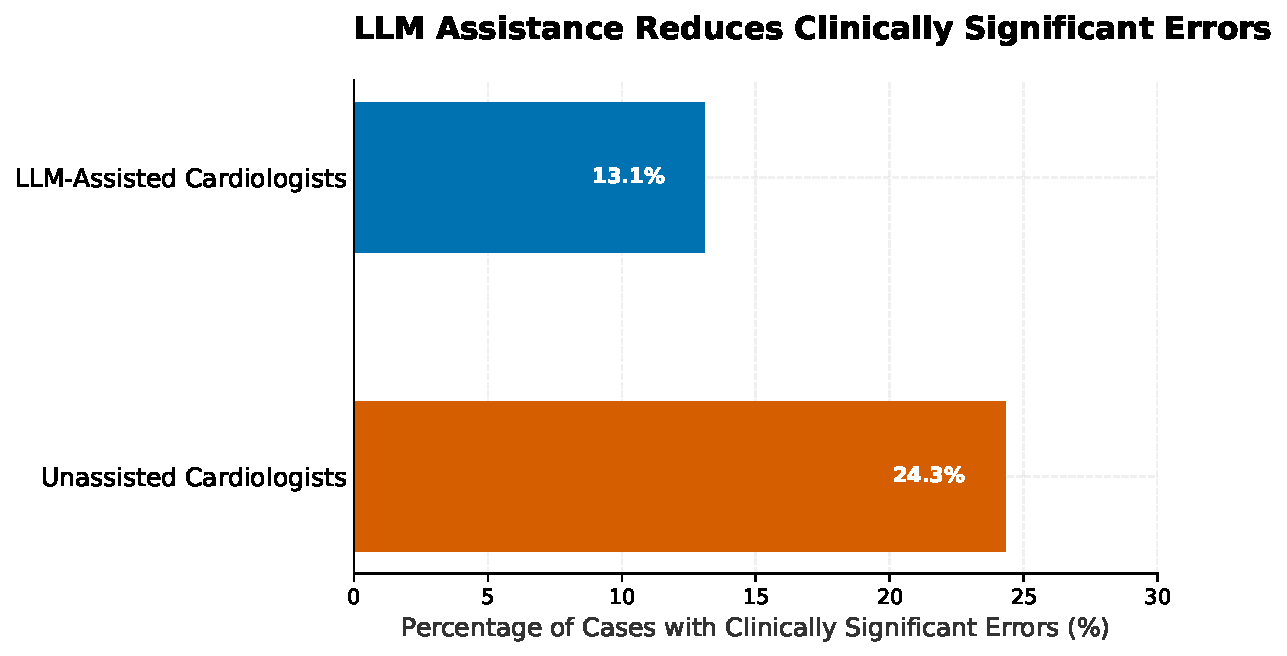
\includegraphics[width=\textwidth]{error_reduction.pdf}
        \caption{Reduction in Errors}
        \label{fig:error}
    \end{subfigure}
    \hfill
    \begin{subfigure}[b]{0.45\textwidth}
        \centering
        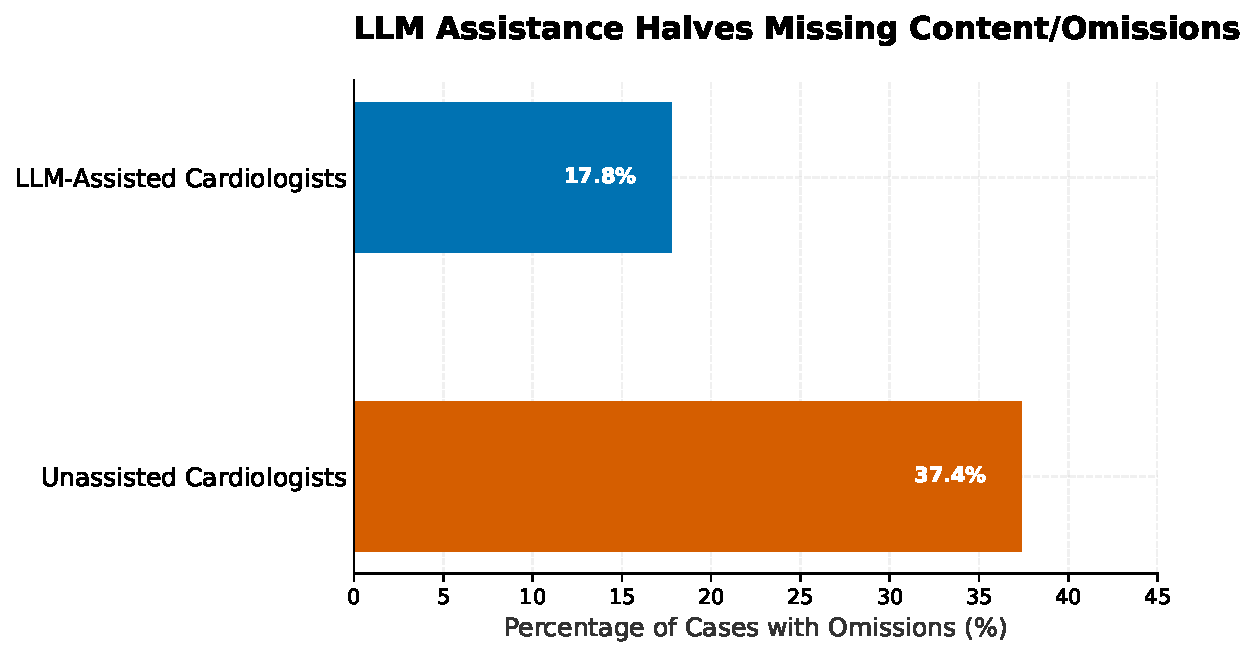
\includegraphics[width=\textwidth]{omission_reduction.pdf}
        \caption{Reduction in Omissions}
        \label{fig:omission}
    \end{subfigure}
    \caption{Baseline efficacy of LLM assistance in cardiology. (a) LLM-assisted assessments exhibited a dramatic reduction in clinically significant errors (13.1\% vs. 24.3\%, $P=0.033$). (b) Missing content and omissions were halved (17.8\% vs. 37.4\%, $P=0.0021$).}
    \label{fig:baseline_errors}
\end{figure}

Furthermore, when evaluating the overall management plans for complex cardiovascular disease, subspecialist experts vastly preferred the plans generated with LLM assistance.

\begin{figure}[H]
    \centering
    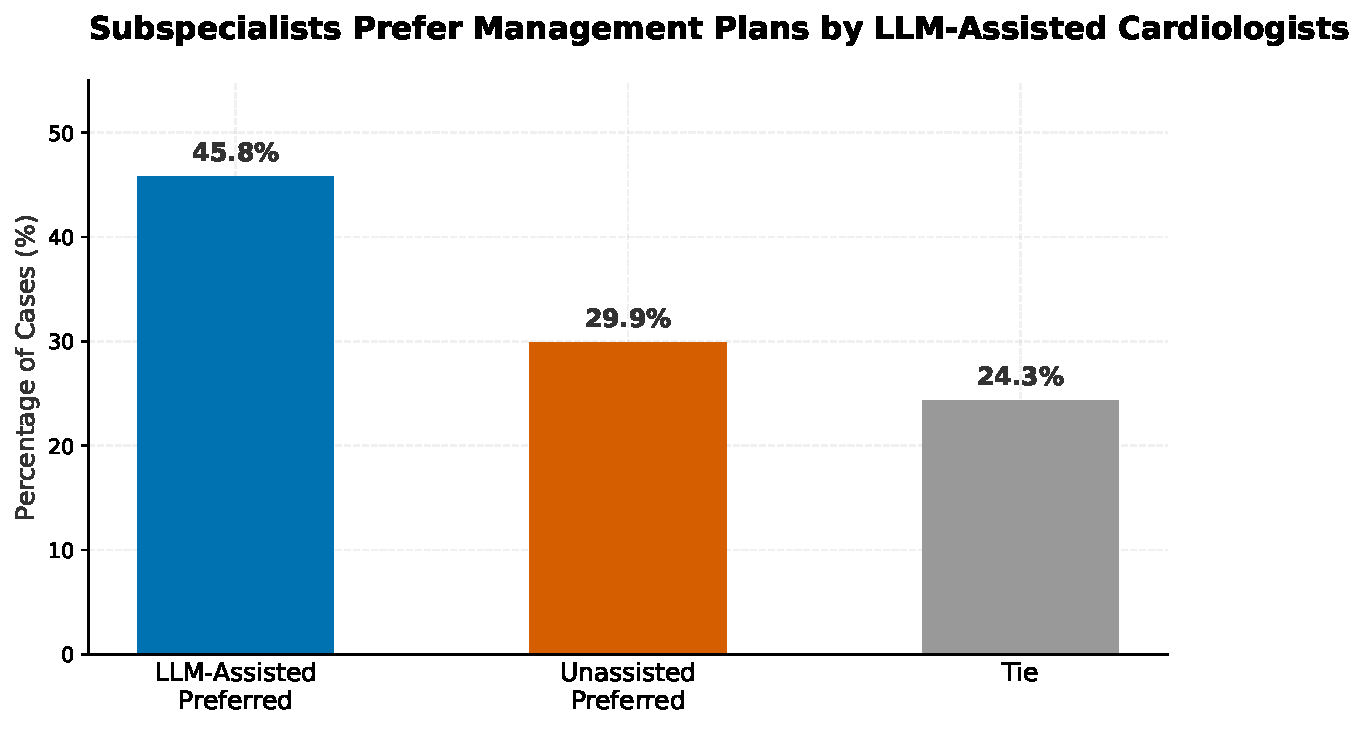
\includegraphics[width=0.6\textwidth]{management_preference.pdf}
    \caption{Subspecialist preference for management plans generated by LLM-assisted vs. unassisted cardiologists ($P=0.008$).}
    \label{fig:preference}
\end{figure}

These baseline results categorically validate the clinical utility of specialized LLMs in cardiology. Cardio-Sahayak builds upon these findings, expecting equivalent or superior performance specifically on South Asian clinical vignettes.

\subsection{Cardio-Sahayak Evaluation Protocol}
The v0 iteration of Cardio-Sahayak undergoes a strict evaluation pipeline (implemented via \texttt{modal\_eval\_cardio\_sahayak.py}) leveraging the EleutherAI LM Evaluation Harness:
\begin{enumerate}
    \item \textbf{Standardized Benchmarks:} Initial evaluation is performed against standard medical QA datasets, including MedQA (USMLE-style questions) and PubMedQA.
    \item \textbf{Demographic-Specific Testing:} Evaluation against a proprietary hold-out set of Indian clinical case studies to measure the model's adherence to Indian clinical guidelines.
    \item \textbf{Multimodal Concordance:} Measuring the accuracy of the VLM against cardiologist-annotated 12-lead ECG benchmarks.
\end{enumerate}

\section{Limitations}
While promising, Cardio-Sahayak India currently faces several limitations:
\begin{itemize}
    \item \textbf{Retrospective Data Bias:} The initial fine-tuning relies on retrospective text datasets, which may contain inherent diagnostic biases.
    \item \textbf{Hallucination Risks:} Despite QLoRA fine-tuning, large language models remain susceptible to hallucinations, especially when faced with conflicting multimodal inputs (e.g., discrepancies between echo and MRI reports). The model must be deployed strictly as a "Sahayak" (assistant) with human-in-the-loop oversight.
    \item \textbf{Pending Prospective RCTs:} The demographic-specific efficacy requires validation through a prospective, multi-center RCT in Indian hospitals to guarantee real-world safety.
\end{itemize}

\section{Conclusion and Future Work}
Cardio-Sahayak India represents a targeted, open-source effort to democratize expert-level cardiology care for the South Asian demographic. By combining state-of-the-art multimodal Large Language Models, parameter-efficient fine-tuning via Modal.com, and specific contextualization for the South Asian Phenotype, this project provides a highly scalable solution to the cardiology workforce crisis in India. All model weights and adapters have been open-sourced on Hugging Face (\texttt{tp53/cardio-sahayak} and \texttt{tp53/cardio-sahayak-vlm}) under a CC-BY-4.0 license.

Future work will focus on converting these merged models into GGUF formats (via \texttt{modal\_gguf\_convert.py}) for efficient, low-resource edge deployment in rural clinics, and on executing rigorous prospective clinical trials.

\begin{thebibliography}{9}
\bibitem{AMIE2026}
Tu, T., et al. (2026). \textit{A large language model for complex cardiology care}. Nature Medicine, 32, 616--623.

\bibitem{EchoJEPA2025}
Authors. (2025). \textit{EchoJEPA: A Latent Predictive Foundation Model for Echocardiography}. 

\bibitem{ECGJEPA2024}
Authors. (2024). \textit{Learning General Representation of 12-Lead ECG with a Joint-Embedding Predictive Architecture}.
\end{thebibliography}

\end{document}